\bibliographystyle{ieeetr}
\documentclass[letterpaper, 10 pt, conference]{ieeeconf}
%\documentclass[12pt,onecolumn,draftcls]{IEEEtran}
%\documentclass[journal]{IEEEtran}


\usepackage{here}
\usepackage{graphicx}
\usepackage[outdir=./]{epstopdf}
\DeclareGraphicsExtensions{.eps}
\usepackage{subfigure}
\usepackage{cite}
\usepackage{bm}
\usepackage{stfloats}

\def\vec#1{\mbox{\boldmath $#1$}}

\IEEEoverridecommandlockouts                              % This command is only
                                                          % needed if you want to
                                                          % use the \thanks command
\overrideIEEEmargins

\title{\LARGE \bf A Synchronization Scheme for Position Control of Multiple Rope-Climbing Robots}
\author{
\thanks{The authors are with the Department of Mechanical and Automation
Engineering, The Chinese University of Hong Kong, Hong Kong S.A.R.
This work was
supported by the HK RGC under Grant no. 415011 and
CUHK6/CRF/13G.}}

\begin{document}
\maketitle

\begin{abstract}
%Compared with stiff actuators, compliant actuators are known to
%offer a range of advantages such as high force fidelity, low output
%impedance, and tolerance to shocks, and its application can be found in
%both industry and healthcare.
The dynamic model of rope-climbing robot
consisting both the robot dynamics and the actuator dynamics is
a high-order system with couplings between each other, which opens
up challenges in the development of robot control schemes.
%While several progress has been achieved in the control of
%compliantly actuated robots, the open issue of safety has not been
%systematically addressed.
This paper presents an adaptive control scheme for the synchronization task among multiple rope-climbing robots.
The stability of closed-loop system is rigorously proved with
Lyapunov methods, with the consideration of both the robot
dynamics and the actuator dynamics.
Experimental results are
presented to validate the proposed controller.
\end{abstract}
\begin{keywords}climbing robots, motion control.\end{keywords}

\section{Introduction}
The overall rope-climbing robotic system
consisting both the robot dynamics and the actuator dynamics,
is a high-order system with couplings between each other. Hence, controllers for rope-climbing robots should be
able to stabilize both subsystems, and neglecting the coupling
dynamics is exposed to stability issues \cite{ram15_petit}.

Few results have been reported in the literature for the position control of rope-climbing robot. Existing results are limited to a single robot, and not applicable to the coordination between multiple robots. Some applications require the synchronization control of multiple rope-climbing robots.

In this paper, an adaptive controller is proposed to address the synchronization problem of multiple rope-climbing robots.
The stability of closed-loop system is rigorously proved with
Lyapunov methods, by taking into account the dynamics of both the
robot subsystem and the actuator subsystem. The uncertain dynamic parameters are updated with online adaptation laws. Experimental results are presented to validate the proposed controller.

\section{Background}

\subsection{Mechanical Structure}
-- briefly introduce the structure --
%\begin{center}
%\begin{figure}[h]
%\centering
%\includegraphics[width=2.9in]{NewActuator_4_4.eps}
%\caption{Mechanical structure of the compliant actuator: (a)
%Principle of the actuator design (CAD model); (b)
%Prototype.}\label{compliantActuator}
%\end{figure}
%\vspace{-0.5cm}
%\end{center}

\subsection{Dynamic Model}
The overall dynamic model of a rope-climbing robot consists of two subsystems: the robot and the actuator.
In the following analysis, the rotary elements of the rope-climbing robot are converted to equivalent translational elements,
without loss of generality. Considering $n$ rope-climbing robots,
the overall dynamic model can be
described as \cite{ram15_petit}:
\begin{eqnarray}
&\bm M\ddot{{\bm q}}\hspace{-0.05cm}+\hspace{-0.05cm}\bm
D \dot{\bm q}\hspace{-0.05cm}+\hspace{-0.05cm}\bm
G\hspace{-0.05cm}=\hspace{-0.05cm}\bm K(\bm
\theta\hspace{-0.05cm}-\hspace{-0.05cm}\bm
q),\label{grobotDyn}\\
&\bm B\ddot{\bm \theta}\hspace{-0.05cm}+\hspace{-0.05cm}\bm K(\bm
\theta\hspace{-0.05cm}-\hspace{-0.05cm}\bm q)=\bm
u,\label{gactuatorDyn}
\end{eqnarray}
where $\bm q\hspace{-0.1cm}=\hspace{-0.1cm}[q_1, \cdots, q_n]^T\hspace{-0.1cm}\in\hspace{-0.1cm}\Re^n$ is the vector of
robot displacement, $q_i$ $(i\hspace{-0.1cm}=\hspace{-0.1cm}1, \cdots, n)$ is the displacement of the $i^{th}$ robot, $\bm
\theta\hspace{-0.1cm}\in\hspace{-0.1cm}\Re^n$ is the vector of motor displacement, $\theta_i$ is the displacement of the $i^{th}$ motor, $\bm M\hspace{-0.1cm}=\hspace{-0.1cm}{\rm diag}(M_1, \cdots, M_n)\hspace{-0.1cm}\in\hspace{-0.1cm}\Re^{n\times n}$ is the diagonal mass matrix of robot where $M_i$ are positive constants, $\bm D\hspace{-0.1cm}=\hspace{-0.1cm}{\rm diag}(D_1, \cdots, D_n)\hspace{-0.1cm}\in\hspace{-0.1cm}\Re^{n\times n}$ denotes the diagonal friction matrix where $D_i$ are also positive constants, and
$\bm G\hspace{-0.1cm}\in\hspace{-0.1cm}\Re^n$ is the gravity matrix, $\bm
K\hspace{-0.1cm}=\hspace{-0.1cm}{\rm diag}(K_1, \cdots, K_n)\hspace{-0.1cm}\in\hspace{-0.1cm}\Re^{n\times n}$ denotes the
stiffness matrix where $K_i$ is the stiffness of the $i^{th}$ rope,
$\bm B
\hspace{-0.1cm}=\hspace{-0.1cm}{\rm diag}(B_1, \cdots, B_n)\hspace{-0.1cm}\in\hspace{-0.1cm}\Re^{n\times n}$ is the diagonal mass matrix of actuator, and $\bm
u\hspace{-0.1cm}\in\hspace{-0.1cm}\Re^n$ denotes the input forces
exerted on actuators.

Equation (\ref{grobotDyn}) describes the well-known rigid-body dynamics, and equation (\ref{gactuatorDyn}) describes the actuator dynamics. The two subsystems are linked to each other with the stretching force of the rope, i.e. $\bm K(\bm\theta-\bm q)$.
In this paper, it is assumed the dynamic models for the robot and actuator are well defined, that is, $\bm M$, $\bm D$, $\bm G$, $\bm B$, and $\bm K$ are exactly known.  %that the stiffness $\bm K$ and the
%mass matrix $\bm B$ of actuator are assumed to be well defined,
%while other dynamic parameters, i.e. $\bm M$, $\bm D$, and $\bm G$, are unknown and will be estimated
%by on-line adaptation laws. %Note that the first three terms of (\ref{grobotDyn}) are linear in a
%set of physical parameters
%as:
%\begin{eqnarray}
%&\bm M\ddot{{\bm q}}\hspace{-0.05cm}+\hspace{-0.05cm}\bm
%D\dot{\bm q}\hspace{-0.05cm}+\hspace{-0.05cm}\bm
%G\hspace{-0.05cm}=\hspace{-0.05cm}\bm Y_q(\dot{\bm q}, \ddot{\bm q})\bm\psi_q,
%\end{eqnarray}
%where $\bm\psi_q\hspace{-0.05cm}=\hspace{-0.05cm}[\psi_{q1}, \cdots,
%\psi_{qn_q}]^T\hspace{-0.05cm}\in\hspace{-0.05cm}\Re^{n_q}$ is the vector of dynamic parameters, and $\bm Y_q(\dot{\bm q}, \ddot{\bm
%q})\hspace{-0.1cm}\in\hspace{-0.1cm}\Re^{n\times n_q}$ is a known
%dynamic regressor matrix.

\section{Synchronization Scheme For Multiple Rope-Climbing Robots}
The mechanical dynamics of robot is slower
(\ref{grobotDyn}) while the dynamics of robot is faster (\ref{gactuatorDyn}), and hence the overall rope-climbing robotic system
exhibits the features of two time scales
\cite{automatica95_spong}. In this paper, the singular perturbation
theory \cite{khalil} is introduced to design controllers for two
subsystems separately, by treating the faster dynamics as
perturbation of the slower dynamics.

\subsection{Controller for Actuator Subsystem}

The overall controller for multiple rope-climbing robots can be proposed as:
\begin{eqnarray}
&\bm u\hspace{-0.05cm}=\hspace{-0.05cm}\bm u_s+\bm
u_f,\label{overall}
\end{eqnarray}
where $\bm u_s, \bm u_f\hspace{-0.1cm}\in\hspace{-0.1cm}\Re^n$
represent the slow controller for the robot subsystem and the fast controller for the actuator subsystem respectively.

First,
the fast controller is specified as:
\begin{eqnarray}
&\bm
u_f\hspace{-0.05cm}=\hspace{-0.05cm}-\bm K_v(\dot{\bm
\theta}\hspace{-0.05cm}-\hspace{-0.05cm}\dot{\bm q}),\label{fastControl}
\end{eqnarray}
where $\bm
K_v\hspace{-0.1cm}\in\hspace{-0.1cm}\Re^{n\times n}$ is a diagonal
and positive-definite matrix. Substituting (\ref{overall}) into
(\ref{gactuatorDyn}) yields:
\begin{eqnarray}
&\bm B\ddot{\bm \theta}\hspace{-0.05cm}+\hspace{-0.05cm}\bm
K_v(\dot{\bm \theta}\hspace{-0.05cm}-\hspace{-0.05cm}\dot{\bm
q})\hspace{-0.05cm}+\hspace{-0.05cm}\bm K\hspace{-0.00cm}(\bm
\theta\hspace{-0.05cm}-\hspace{-0.05cm}\bm
q)\hspace{-0.1cm}=\hspace{-0.1cm}\bm u_s,
\end{eqnarray}
which leads to:
\begin{eqnarray}
&\bm B(\ddot{\bm \theta}\hspace{-0.05cm}-\hspace{-0.05cm}\ddot{\bm
q})\hspace{-0.05cm}+\hspace{-0.05cm}\bm K_v(\dot{\bm
\theta}\hspace{-0.05cm}-\hspace{-0.05cm}\dot{\bm
q})\hspace{-0.05cm}+\hspace{-0.05cm}\bm K\hspace{-0.00cm}(\bm
\theta\hspace{-0.05cm}-\hspace{-0.05cm}\bm
q)\hspace{-0.05cm}=\hspace{-0.05cm}\bm
u_s\hspace{-0.05cm}-\hspace{-0.05cm}\bm B\ddot{\bm q}.\label{temp11}
\end{eqnarray}

Next, a variable $\bm y$ is introduced as the stretching force of the rope as: $\bm y\hspace{-0.05cm}=\hspace{-0.05cm}\bm K(\bm
\theta\hspace{-0.05cm}-\hspace{-0.05cm}\bm q)$, such that equations
(\ref{grobotDyn}) and (\ref{temp11}) can be written as:
\begin{eqnarray}
&\bm M\ddot{{\bm q}}\hspace{-0.05cm}+\hspace{-0.05cm}\bm
D\dot{\bm q}\hspace{-0.05cm}+\hspace{-0.05cm}\bm
G\hspace{-0.05cm}=\hspace{-0.05cm}\bm
y,\label{robotDyn2}\\
&\bm B\ddot{\bm y}\hspace{-0.05cm}+\hspace{-0.05cm}\bm K_v\dot{\bm
y}\hspace{-0.05cm}+\hspace{-0.05cm}\bm K\bm
y\hspace{-0.1cm}=\hspace{-0.1cm}\bm K(\bm
u_s\hspace{-0.05cm}-\hspace{-0.05cm}\bm B\ddot{\bm
q}).\label{temp21}
\end{eqnarray}
Expressing $\bm K$ and $\bm K_v$ in terms of $\epsilon$ as
\cite{automatica95_spong}:
\begin{eqnarray}
&\bm K=\bm K_1/\epsilon^2,\\
&\bm K_v=\bm
K_2/\epsilon,
\end{eqnarray}
where $\epsilon$ is a small parameter. Then, equation
(\ref{temp21}) becomes:
\begin{eqnarray}
&\epsilon^2\bm B\ddot{\bm
y}\hspace{-0.05cm}+\hspace{-0.05cm}\epsilon\bm K_2\dot{\bm
y}\hspace{-0.05cm}+\hspace{-0.05cm}\bm K_1\bm
y\hspace{-0.1cm}=\hspace{-0.1cm}\bm K_1(\bm
u_s\hspace{-0.05cm}-\hspace{-0.05cm}\bm B\ddot{\bm
q}).\label{temp31}
\end{eqnarray}
The system described by (\ref{robotDyn2}) and (\ref{temp31}) is
singularly perturbed. The variables $\bm y$ and $\dot{\bm y}$ can be
viewed as fast time-scale variables, while the state variables ${\bm
q}$ and $\dot{\bm q}$ denote slow time-scale variables.

With
$\epsilon\hspace{-0.05cm}=\hspace{-0.05cm}0$, equation
(\ref{temp31}) becomes:
\begin{eqnarray}
&\bar{\bm y}\hspace{-0.05cm}=\hspace{-0.05cm}{\bm u}_s-\bm
B\ddot{{\bm q}},\label{solution}
\end{eqnarray}
in which, the overbar variable denotes the value of variable at
$\epsilon\hspace{-0.1cm}=\hspace{-0.1cm}0$. Then, substituting
equation (\ref{solution}) into equation (\ref{robotDyn2}) at
$\epsilon\hspace{-0.1cm}=\hspace{-0.1cm}0$ yields the {\em
quasi-steady-state} model:
\begin{eqnarray}
&(\bm M\hspace{-0.05cm}+\hspace{-0.05cm}\bm B)\ddot{{{\bm
q}}}\hspace{-0.05cm}+\hspace{-0.05cm}\bm D\dot{{\bm q}}\hspace{-0.05cm}+\hspace{-0.05cm}\bm G\hspace{-0.05cm}=\hspace{-0.05cm}{\bm
u}_s.\label{quasi}
\end{eqnarray}

By assuming that $\bar{\bm y}$ is constant on a fast time-scale
$\tau\hspace{-0.05cm}=\hspace{-0.05cm}\frac{t}{\epsilon}$, a new
variable is introduced as:
$\bm\eta\hspace{-0.05cm}=\hspace{-0.05cm}\bm
y\hspace{-0.05cm}-\hspace{-0.05cm}\bar{\bm y}$. Substituting the
fast time-scale $\tau$ and $\bm y=\bm\eta+\bar{\bm y}$ into
(\ref{temp31}), with $\frac{{\rm d}\bar{\bm y}}{{\rm
d}\tau}=\frac{{\rm d}^2\bar{\bm y}}{{\rm d}\tau^2}=\bm 0$ and
$\epsilon=0$, we have:
\begin{eqnarray}
&\bm B(\frac{{\rm d}^2\bm\eta}{{\rm
d}\tau^2})\hspace{-0.05cm}+\hspace{-0.05cm}\bm K_2(\frac{{\rm
d}\bm\eta}{{\rm d}\tau})\hspace{-0.1cm}+\hspace{-0.1cm}\bm
K_1\bm\eta\hspace{-0.05cm}=\hspace{-0.05cm}\bm 0,\label{boundary}
\end{eqnarray}
which is referred to as {\em boundary-layer system}.

According to
Tikhonov's theorem \cite{khalil}, the overall system is stable if
both the {\em boundary-layer system} (\ref{boundary}) and the {\em
quasi-steady-state system} (\ref{quasi}) are exponentially stable.
The exponential stability of the {\em boundary-layer system} can be
guaranteed by specifying $\bm K_1$ and $\bm K_2$ from
(\ref{boundary}). Then, the control objective is to design a slow
controller $\bm u_s$ which guarantees the exponential stability of
the {\em quasi-steady-state system} (\ref{quasi}).

\subsection{Controller for Robot Subsystem}
In this section, a slow controller $\bm u_s$ is specified such that the {\em quasi-steady-state system} is exponentially stable. The slow controller also guarantees the convergence of the position of each robot to the desired position, and achieves the synchronization between each other. %an adaptive controller is proposed for
%the synchronization task of multiple rope-climbing robots, by stabilizing both the actuator
%subsystem and the robot subsystem. %The development of the
%proposed controller follows a backstepping approach. That is, based
%on the dynamics of the robot subsystem, a fictitious desired
%input $\bm\theta_d$ is proposed to achieve the synchronization. Next, based on the dynamics of the actuator subsystem, the
%control input $\bm u$ is derived to realize the fictitious signal,
%such that the actual shaft position of actuator $\bm\theta$ tracks
%the desired input $\bm\theta_d$.

First, a sliding vector is introduced as:
\begin{eqnarray}
&\bm s\hspace{-0.05cm}=\hspace{-0.05cm}\dot{\bm
q}\hspace{-0.05cm}-\hspace{-0.05cm}\dot{\bm
q}_r\hspace{-0.05cm}=\hspace{-0.05cm}\dot{\bm
q}\hspace{-0.05cm}-\hspace{-0.05cm}\dot{\bm q}_d+\alpha_q\Delta\bm q+\alpha_s\Delta\bm\psi,\label{imCon1}
\end{eqnarray}
where
\begin{eqnarray}
&\dot{\bm q}_r\hspace{-0.05cm}=\hspace{-0.05cm}\dot{\bm q}_d-\alpha_q\Delta\bm q-\alpha_s\Delta\bm\psi,\label{xo}
\end{eqnarray}
is a reference vector, $\alpha_q$ and $\alpha_s$ are positive constants, $\Delta\bm q=\bm q-\bm q_d$ where $\bm q_d\hspace{-0.05cm}=\hspace{-0.05cm}[q_{d1}, \cdots, q_{dn}]\hspace{-0.05cm}\in\hspace{-0.05cm}\Re^n$ denotes the vector of desired positions, $q_{di}$ is the desired position for the $i$th robot, and $\Delta\bm\psi$ denotes the synchronization vector which is specified as:
$\Delta\bm\psi\hspace{-0.05cm}=\hspace{-0.05cm}[\psi_1-\psi_n, \psi_2-\psi_1, \cdots, \psi_n-\psi_{n-1}]^T$ where $\psi_1=\Delta q_1-\Delta q_2$, $\cdots$, $\psi_n=\Delta q_n-\Delta q_1$. The definition of synchronization errors was introduced in \cite{sdtmech}, We can now propose the slow controller $\bm u_s$ as:
\begin{eqnarray}
&\bm u_s\hspace{-0.05cm}=\hspace{-0.05cm}-\bm K_s\bm
s\hspace{-0.05cm}-\hspace{-0.05cm}k_q\Delta\bm q\hspace{-0.05cm}+\hspace{-0.05cm}(\bm{M}+\bm B)\ddot{\bm
q}_r\hspace{-0.05cm}+\hspace{-0.05cm}\bm D\dot{\bm
q}_r+\bm G,\label{thd}
\end{eqnarray}
where $\bm K_s\hspace{-0.05cm}\in\hspace{-0.05cm}\Re^{n\times n}$ is
positive-definite, and $k_q$ is a positive constant. In (\ref{thd}), the first two terms include the position control, the synchronization control, and the velocity control, and the last three terms represent the dynamic compensation.

The key novelty of the proposed control method is to integrate both the position error $\Delta\bm q$ and the synchronization error $\Delta\bm\varepsilon$ into a single controller, such that multiple robots can move to the desired positions while always maintaining the same height when they are climbing along the ropes. Both the position control task and the synchronization control task are important for the coordination of multiple rope-climbing robots. For example, when a manipulator is installed at the center of multiple rope-climbing robots and the vertical position of the manipulator is varied by controlling the multiple robots as shown in Fig. \ref{??}, the proposed control method allows the manipulator to be transported to a desired vertical position to perform manipulation tasks (e.g. wiping the window), and also guarantees that the base of the manipulator is always parallel to the ground throughout the transportation.

Note that the overall dynamic model described by (\ref{grobotDyn}) and (\ref{gactuatorDyn}) is a high-order system, while the complexity of the proposed controller in (\ref{overall}) is the same as that of the dynamics of the robot subsystem. That is, the use of singular perturbation approach helps to decrease the complexity and also the computational const of the controller.

By using the sliding vector (\ref{imCon1}), the dynamics of the {\em quasi-steady-state system}
can be rewritten as:
\begin{eqnarray}
&(\bm{M}+\bm B)\dot{\bm s}\hspace{-0.05cm}+\hspace{-0.05cm}\bm D\bm
s\hspace{-0.05cm}+\hspace{-0.05cm}(\bm{M}+\bm B)\ddot{\bm
q}_r\hspace{-0.05cm}+\hspace{-0.05cm}\bm D\dot{\bm
q}_r+\bm G=\bm u_s.\label{taskDyn2}
\end{eqnarray}
%where
%$\Delta\bm\theta\hspace{-0.05cm}=\hspace{-0.05cm}\bm\theta\hspace{-0.05cm}-\hspace{-0.05cm}\bm\theta_d$.
%The desired input $\bm\theta_d$ is considered as a fictitious input
%for the robot, and $\Delta\bm\theta$ represents an input
%perturbation to the robot dynamics. The system in (\ref{taskDyn2})
%can be viewed as being controlled by the input $\bm K\bm \theta_d$
%with the perturbation of $\bm K\Delta\bm\theta$.
%
%Equation (\ref{taskDyn2}) can also be written
%as:
%\begin{eqnarray}
%&\bm{M}\dot{\bm s}\hspace{-0.05cm}+\hspace{-0.05cm}\bm D\bm s\hspace{-0.05cm}+\hspace{-0.05cm}\bm Y_q(\dot{\bm q}_r, \ddot{\bm
%q}_r)\bm\psi_q\hspace{-0.05cm}+\hspace{-0.05cm}\bm K\bm q=\bm K\bm \theta_d\hspace{-0.05cm}+\hspace{-0.05cm}\bm
%K\Delta\bm\theta.\label{taskDyn3}
%\end{eqnarray}

Substituting (\ref{thd}) into (\ref{taskDyn2})
yields the following dynamic equation:
\begin{eqnarray}
&(\bm{M}+\bm B)\dot{\bm
s}\hspace{-0.1cm}+\hspace{-0.1cm}(\bm D\hspace{-0.1cm}+\hspace{-0.1cm}\bm K_s)\bm
s\hspace{-0.1cm}+\hspace{-0.1cm}k_q\Delta\bm q=\bm
0.\label{robotclosed1}
\end{eqnarray}
%where
%$\Delta{\bm\psi}_q\hspace{-0.05cm}=\hspace{-0.05cm}\bm\psi_q\hspace{-0.05cm}-\hspace{-0.05cm}\hat{\bm\psi}_q$.

%\subsection{Control Input for Compliant Actuator}
%In this section, the control input for the actuator $\bm u$ is
%developed such that the actual position of the actuator $\bm\theta$
%track the desired input $\bm\theta_d$ and hence
%$\Delta\bm\theta\hspace{-0.05cm}\rightarrow\hspace{-0.05cm}\bm 0$.
%First, a sliding vector is introduced for actuator as:
%\begin{eqnarray}
%&{\bm s}_{\theta}\hspace{-0.05cm}=\hspace{-0.05cm}\dot{\bm
%\theta}\hspace{-0.05cm}-\hspace{-0.05cm}\dot{{\bm
%\theta}}_r\hspace{-0.05cm}=\hspace{-0.05cm}\dot{\bm
%\theta}\hspace{-0.05cm}-\hspace{-0.05cm}\dot{{\bm
%\theta}}_d\hspace{-0.05cm}+\hspace{-0.05cm}\alpha_{\theta}({\bm
%\theta}\hspace{-0.05cm}-\hspace{-0.05cm}{{\bm
%\theta}}_d)\hspace{-0.05cm}=\hspace{-0.05cm}\Delta\dot{{\bm\theta}}\hspace{-0.05cm}+\hspace{-0.05cm}\alpha_{\theta}\Delta{{\bm\theta}}.
%\end{eqnarray}
%where  $\alpha_{\theta}$ is a positive constant, and $\dot{{\bm
%\theta}}_r$ is a reference vector which is defined as:
%\begin{eqnarray}
%&\dot{{\bm \theta}}_r=\dot{{\bm
%\theta}}_d-\alpha_{\theta}\Delta{\bm\theta}.\label{dbqr}
%\end{eqnarray}
%
%The control input of the actuator is now proposed as:
%\begin{eqnarray}
%&{\bm u}\hspace{-0.05cm}=\hspace{-0.05cm}\bm K({\bm
%\theta}\hspace{-0.05cm}-\hspace{-0.05cm}\bm
%q)\hspace{-0.05cm}-\hspace{-0.05cm}\bm K_{\theta}{\bm
%s}_{\theta}\hspace{-0.05cm}+\hspace{-0.05cm}\bm B\ddot{{\bm
%\theta}}_r,\label{MotorControl}
%\end{eqnarray}
%where $\bm K_{\theta}$ is a positive definite matrix. Using the
%sliding vector ${\bm s}_{\theta}$, equation (\ref{gactuatorDyn}) is
%expressed as:
%\begin{eqnarray}
%&\bm B\dot{{\bm s}}_{\theta}\hspace{-0.05cm}+\hspace{-0.05cm}\bm
%K(\bm\theta\hspace{-0.05cm}-\hspace{-0.05cm}\bm
%q)\hspace{-0.05cm}+\hspace{-0.05cm}\bm B\ddot{{\bm \theta}}_r=\bm
%\tau.\label{dmotor2}
%\end{eqnarray}
%
%Substituting (\ref{MotorControl}) into (\ref{dmotor2}), the
%closed-loop equation of the compliantly actuated robot is obtained
%as:
%\begin{eqnarray}
%&\hspace{-0.2cm}\bm B\dot{{\bm
%s}}_{\theta}\hspace{-0.05cm}+\hspace{-0.05cm}\bm K_{\theta}{\bm
%s}_{\theta}\hspace{-0.05cm}=\hspace{-0.05cm}\bm 0,\label{ntemp7}
%\end{eqnarray}
%which clearly shows the convergence of $\bm
%s_{\theta}\hspace{-0.05cm}\rightarrow\hspace{-0.05cm}\bm 0$, and
%thus $\Delta\bm\theta\hspace{-0.05cm}\rightarrow\hspace{-0.05cm}\bm
%0$.

Now we are in the position to state the following theorem.\\
\textbf{Theorem}: {\em The proposed controller
described by (\ref{overall}), (\ref{fastControl}), and (\ref{thd})
for multiple rope-climbing robots guarantees the stability of the closed-loop system and the convergence of tracking errors and synchronization errors to zero, if the control parameters are chosen such that
\begin{eqnarray}
&\lambda_{\min}[\bm K_s]\geq\lambda_{\max}[\frac{1}{2}(\bm M+\bm B)-\bm D],\label{con1}\\
&\alpha_q\geq\frac{1}{2},\label{con2}
\end{eqnarray}
where $\lambda_{\min}[\cdot]$ and $\lambda_{\max}[\cdot]$ represent the minimum and the maximum eigenvalues respectively.
}

\begin{proof}
A Lyapunov-like candidate is proposed as:
\begin{eqnarray}
&V\hspace{-0.05cm}=\hspace{-0.05cm}\frac{1}{2}\bm s^T(\bm M\hspace{-0.05cm}+\hspace{-0.05cm}\bm B)\bm
s\hspace{-0.05cm}+\hspace{-0.05cm}\frac{k_q}{2}\Delta\bm q^T\Delta\bm q.\label{Lya}
\end{eqnarray}

Differentiating (\ref{Lya}) with respect to time yields:
\begin{eqnarray}
&\dot V\hspace{-0.05cm}=\hspace{-0.05cm}\bm s^T(\bm M\hspace{-0.05cm}+\hspace{-0.05cm}\bm B)\dot{\bm
s}\hspace{-0.05cm}+\hspace{-0.05cm}k_q\Delta\bm q^T\Delta\dot{\bm q}.\label{dLya}
\end{eqnarray}

Substituting (\ref{imCon1}) and (\ref{robotclosed1}) into
(\ref{dLya}), we have:
\begin{eqnarray}
&\dot V%\hspace{-0.05cm}=\hspace{-0.05cm}-\bm s^T(\bm
%D_q\hspace{-0.05cm}+\hspace{-0.05cm}\bm
%D_{\theta}\hspace{-0.05cm}+\hspace{-0.05cm}\bm K_s)\bm
%s\hspace{-0.05cm}-\hspace{-0.05cm}[\dot{\bm
%q}\hspace{-0.05cm}-\hspace{-0.05cm}{{\bm J}}^+\hspace{-0.05cm}(\bm
%q)\dot{\bm x}_r\nonumber\\
%&+\alpha w(\bm x)\bm J^+\hspace{-0.05cm}(\bm q)\Delta\bm x]^Tw(\bm
%x)\bm J^T(\bm q)\bm
%K_p\Delta\bm x\nonumber\\
%&+\frac{\dot w(\bm x)}{2}\Delta\bm x^T\bm K_p\Delta\bm
%x\hspace{-0.05cm}+\hspace{-0.05cm}w(\bm x)\Delta\bm x^T\bm
%K_p\Delta\dot{\bm x}\nonumber\\
=-\bm s^T(\bm D\hspace{-0.05cm}+\hspace{-0.05cm}\bm K_s)\bm
s-\bm s^T\bm K_q\Delta\bm q\hspace{-0.05cm}+\hspace{-0.05cm}k_q\Delta\bm q^T\Delta\dot{\bm q}\nonumber\\
&=-\bm s^T(\bm D\hspace{-0.05cm}+\hspace{-0.05cm}\bm K_s)\bm
s\hspace{-0.05cm}-\hspace{-0.05cm}\alpha_q k_q\Delta\bm q^T\hspace{-0.05cm}\Delta\bm q\hspace{-0.05cm}-\hspace{-0.05cm}\alpha_s k_q\Delta\bm \psi^T\hspace{-0.05cm}\Delta\bm q.\label{dLya1}
\end{eqnarray}

Note that
\begin{eqnarray}
&\Delta\bm \psi^T\Delta\bm q=\sum\limits_{i=1}^n[\Delta q_i(\psi_i-\psi_{i-1})]\nonumber\\
&=\Delta q_1\psi_1-\Delta q_1\psi_n+\Delta q_2\psi_2-\Delta q_2\psi_1+\cdots\nonumber\\
&+\Delta q_n\psi_n-\Delta q_n\psi_{n-1}\nonumber\\
&=(\Delta q_1-\Delta q_2)\psi_1+(\Delta q_2-\Delta q_3)\psi_2+\cdots\nonumber\\
&+(\Delta q_n-\Delta q_1)\psi_n\nonumber\\
&=\psi_1^2+\psi_2^2+\cdots+\psi_n^2=\bm\psi^T\bm\psi,\label{psi}
\end{eqnarray}
where $\bm\psi=[\psi_1, \cdots, \psi_n]^T\in\Re^n$.

Substituting (\ref{psi}) into (\ref{dLya1}) yields:
\begin{eqnarray}
&\dot V=-\bm s^T(\bm D\hspace{-0.05cm}+\hspace{-0.05cm}\bm K_s)\bm
s\hspace{-0.05cm}-\hspace{-0.05cm}\alpha_q k_q\Delta\bm q^T\hspace{-0.05cm}\Delta\bm q\hspace{-0.05cm}-\hspace{-0.05cm}\alpha_s k_q\bm \psi^T\hspace{-0.05cm}\bm \psi.
\end{eqnarray}
If the control parameters $\bm K_s$ and $\alpha_q$ are chosen such that conditions (\ref{con1}) and (\ref{con2}) are satisfied, it is obtained that
\begin{eqnarray}
&\dot V\leq -\bm s^T(\bm D\hspace{-0.05cm}+\hspace{-0.05cm}\bm K_s)\bm
s\hspace{-0.05cm}-\hspace{-0.05cm}\alpha_q k_q\Delta\bm q^T\hspace{-0.05cm}\Delta\bm q\nonumber\\
&\leq-\gamma
V\hspace{-0.05cm}\leq\hspace{-0.05cm}0,\label{lclosed}
\end{eqnarray}
where $\gamma$ is a positive constant. The inequality
(\ref{lclosed}) indicates that
$V\hspace{-0.05cm}\leq\hspace{-0.05cm}V(0){\rm e}^{-\gamma t}$ where
$V(0)$ denotes the initial value of the Lyapunov-like candidate.
Therefore, the exponential stability of the {\em quasi-steady-state
system} is guaranteed. Since the fast controller (\ref{fastControl}) ensures the exponential
stability of the {\em quasi-steady-state system} (\ref{quasi}), from
the analysis in the previous section, we can also conclude that the
overall controller (\ref{overall}) guarantees the stability of the
rope-climbing robotic system described by (\ref{grobotDyn}) and
(\ref{gactuatorDyn}).

In addition, the
inequality (\ref{lclosed}) implies that $\bm s, \Delta\bm
q\hspace{-0.05cm}\rightarrow\hspace{-0.05cm}\bm 0$ as
$t\hspace{-0.05cm}\rightarrow\hspace{-0.05cm}\infty$. Then, from (\ref{imCon1}), it is obtained that:
\begin{eqnarray}
&\Delta\dot{\bm q}+\alpha_s\Delta \bm\psi\rightarrow\bm 0.\label{temp1}
\end{eqnarray}
In the system of multiple rope-climbing robots, it is usually specified that $q_{d1}=q_{d2}=\cdots=q_{dn}$. Hence, the convergence of $\Delta\bm
q\hspace{-0.05cm}\rightarrow\hspace{-0.05cm}\bm 0$ leads to the convergence of $\Delta\bm
\psi\hspace{-0.05cm}\rightarrow\hspace{-0.05cm}\bm 0$. Then, from (\ref{temp1}), it is concluded that $\Delta\dot{\bm q}\rightarrow\bm 0$.  That is, $\bm q\hspace{-0.05cm}\rightarrow\hspace{-0.05cm}\bm q_d$, 
$\dot{\bm q}\hspace{-0.05cm}\rightarrow\hspace{-0.05cm}\dot{\bm q}_d$, and $q_i\hspace{-0.05cm}\rightarrow\hspace{-0.05cm}q_j$ as $t\hspace{-0.05cm}\rightarrow\hspace{-0.05cm}\infty$. Therefore, the convergence of tracking errors and synchronization errors to zero is guaranteed.
%Next, summing all the error terms yields:
%\begin{eqnarray}
%&\sum\limits_{i=1}^n\Delta\dot{q}+\alpha_s\sum\limits_{i=1}^n\Delta\psi_i\rightarrow 0.\label{temp1}
%\end{eqnarray}
%From the definition of $\Delta\bm\psi$, it is found the second term in (\ref{temp1}) is equal to zero. Therefore, we have:
%\begin{eqnarray}
%&\sum\limits_{i=1}^n\Delta\dot{q}\rightarrow 0.
%\end{eqnarray}
%
% After the robot enters
%the region, $w(\bm x)\hspace{-0.05cm}=\hspace{-0.05cm}0$, and
%(\ref{lclosed}) implies that $\bm
%s\hspace{-0.05cm}\rightarrow\hspace{-0.05cm}\bm 0$ where $\bm
%s\hspace{-0.05cm}=\hspace{-0.05cm}\dot{\bm
%q}\hspace{-0.05cm}-\hspace{-0.05cm}{{\bm J}}^+\hspace{-0.05cm}(\bm
%q)\dot{\bm x}_r$. Therefore, $\dot{\bm
%x}\hspace{-0.05cm}\rightarrow\hspace{-0.05cm}\dot{\bm x}_r$ as
%$t\hspace{-0.05cm}\rightarrow\hspace{-0.05cm}\infty$, and the robot
%is controlled to stay inside the desired region.
\end{proof}

\section{Experiment}
An experimental setup of inspection climbing robot has been established in The Chinese University of Hong Kong.
\begin{figure}[!h]
	\centering
	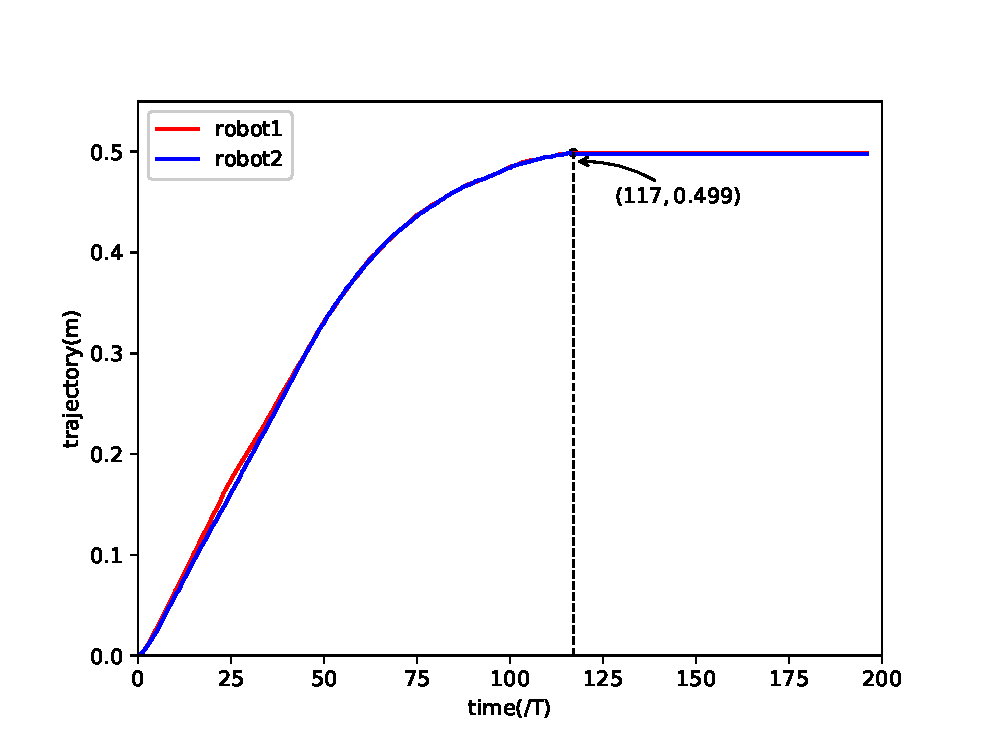
\includegraphics[width=3.4in]{setpoint_trajectory.eps}\label{sp_tr}
	\caption{setpoint control trajectory error of two robots}
\end{figure}	
\begin{figure}[!h]
	\centering
	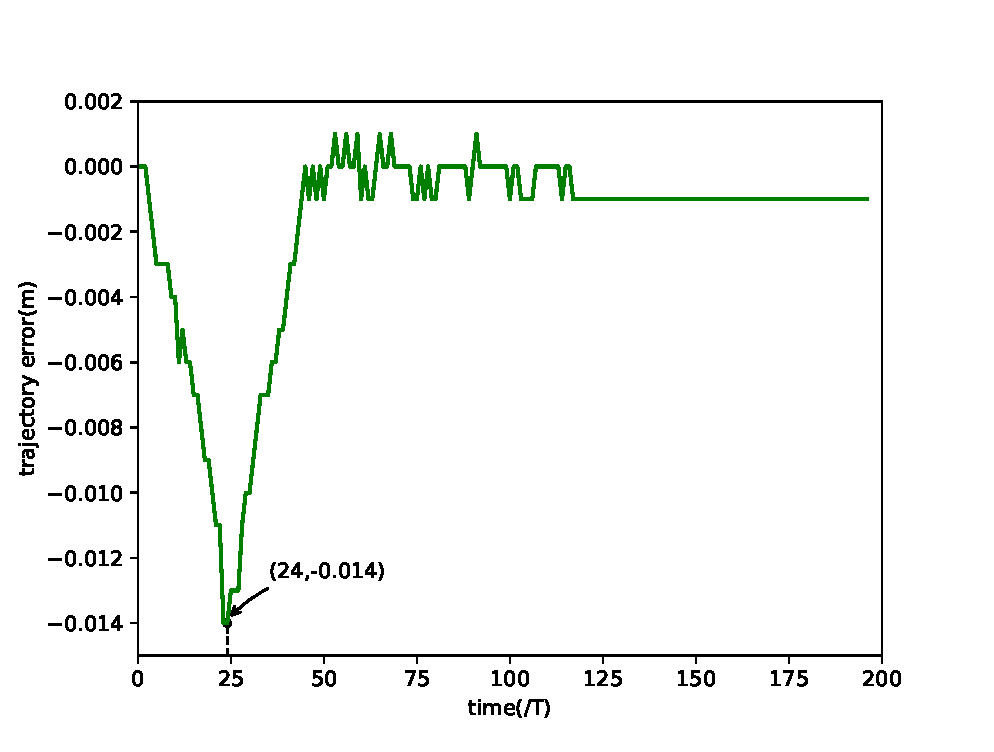
\includegraphics[width=3.4in]{setpoint_error.eps}\label{sp_error}
	\caption{setpoint control trajectory error of two robots}
\end{figure}
%\begin{figure*}[!t]
%  \centering
%  \subfigure[]{
%    \label{SingleTra} %% label for first subfigure
%    \includegraphics[width=3.4in]{icraSingleTra_1_24.eps}}
%  \subfigure[]{
%    \label{SingleErr} %% label for second subfigure
%    \includegraphics[width=3.4in]{icraSingleErr_1_24.eps}}
%  \subfigure[]{
%    \label{SingleForce} %% label for second subfigure
%    \includegraphics[width=3.4in]{icraSingleForce_1_24.eps}}
%  \subfigure[]{
%    \label{SingleIm} %% label for second subfigure
%    \includegraphics[width=3.4in]{icraSingleIm_1_24.eps}}
%  \caption{The controller remains in the {\em Desired-Impedance Mode}.
%  (a) Angular position of robot joint; (b) Position error; (c) Interaction torque; (d) Impedance vector.}
%  \label{Single} %% label for entire figure
%\end{figure*}

\section{Conclusion}

\bibliographystyle{ieeetr}

\begin{thebibliography}{200}
\bibitem{automatica95_spong}
M. W. Spong, "Adaptive control of flexible joint manipulators:
Comments on two papers," {\em Automatica}, 31(4), 585-590, 1995.

\bibitem{khalil}
H. Khalil, \emph{Nonlinear Systems}, Macmillan, New York, 1992.

\bibitem{sdtmech}
Dong Sun, Gang Feng, Chi Ming Lam and Haining Dong, "Orientation control of a differential mobile robot through wheel synchronization," {\em IEEE/ASME Transactions on Mechatronics}, vol. 10, no. 3, pp. 345-351, June 2005.

%\bibitem{tcst16_li}
%X. Li, G. Chi, S. Vidas, and C. C. Cheah, ``Human-guided robotic
%co-manipulation: Two illustrative scenarios,'' \emph{IEEE
%Transactions on Control Systems Technology}, vol. 24, no. 5, pp.
%1751-1763, 2016.
%
%\bibitem{ijrr16_li}
%Y. Pan, G. Chen, and H. Yu, ``Multi-modal control scheme for
%rehabilitation robotic exoskeletons,'' {\em The International
%Journal of Robotics Research}, 2016, in press.
%%%%%%%%%%%%%%%%%%%%%%%%%%%%%%%%%%%
%
%\bibitem{exo2}
%A. M. Dollar and H. Herr, ``Lower extremity exoskeletons and active
%orthoses: challenges and Stage-of-the Art,'' \emph{IEEE Trans.
%Robotics}, vol. 24, no. 1, pp. 144-158, 2008.
%%%%%%%%%%%%%%%%%%%%%%%%%%%%%%%%%
%
%\bibitem{exo1}
%H. Kazerooni, J. L. Racine, L. Huang, and R. Steger, ``On the
%control of the Berkeley Lower Extremity Exoskeleton (BLEEX),''
%\emph{IEEE Int. Conf. Robotics Automat.}, pp. 4353-4360, 2005.
%
%\bibitem{rehabi3}
%H. I. Krebs, B. Volpe, D. Williams, J. Celestino, S. Charles, D.
%Lynch, and N. Hogan, ``Robot-aided neurorehabilitation: a robot for
%wrist rehabilittion,'' \emph{IEEE Trans. Neural Syst. Rehab. Eng.},
%vol. 15, no. 3, pp. 327-335, 2007.
%
%\bibitem{iros95_pratt}%12
%G. A. Pratt and M. M. Williamson, ``Series elastic actuators,''
%\emph{IEEE/RSJ Int. Conf. Intelligent Robots Syst.}, pp. 399-406,
%1995.
%
%\bibitem{ram15_petit}
%F. Petit, A. Dietrich, and A. Albu-Schaffer, ``Generalizing torque
%control concepts: Using well-established torque control methods on
%variable stiffness robots,'' \emph{IEEE Robotics \& Automation
%Magazine}, vol. 22, no. 4, pp. 37-51, 2015.
%
%%%%%%%%%%%%%%%%%%%%%%%%%%%%%%%%%%%%%%%%%%%%%%%%%%%%%%%%%%%%%%%%
%
%\bibitem{jdsmc87_spong}
%M. Spong, ``Modelling and control of elastic joint robots,''
%\emph{Journal of Dynamic Systems, Measurement, and Control}, vol.
%109, pp. 310-319, 1987.
%
%\bibitem{icra92_nicosia}
%S. Nicosia and P. Tomei, ``A method to design adaptive controllers
%for fexible joint robots,'' \emph{IEEE International Conference on
%Robotics and Automation}, pp. 701-706, 1992.
%
%\bibitem{icra98_deluca}
%A. De Luca and P. Lucibello, ``A general algorithm for dynamic
%feedback linearization of robots with elastic joints,'' \emph{IEEE
%International Conference on Robotics and Automation}, pp. 504-510,
%1998.
%
%\bibitem{automatica08_liu}
%C. Liu, C. C. Cheah, and J. J. E. Slotine, ``Adaptive task-space
%regulation of rigid-link flexible-joint robots with uncertain
%kinematics,'' \emph{Automatica}, vol. 44, pp. 1806-1814, 2008.
%
%\bibitem{hogan1}
%N. Hogan, ``Impedance control - An approach to manipulation. I -
%Theory. II - Implementation. III - Applications,'' {\em J. Dyn.
%Syst., Meas., Control}, vol. 107, pp. 1-24, 1985.
%
%\bibitem{hogan2}
%N. Hogan and S. P. Buerger, ``Impedance and interaction control,''
%{\em Robotics and Automation Handbook}. Boca Raton, FL, USA: CRC
%Press, 2001.
%
%\bibitem{ijrr07_albu-schaffer}
%A. Albu-Schaffer, C. Ott, and G. Hirzinger, ``A unified
%passivity-based control framework for position, torque and impedance
%control of flexible joint robots,'' \emph{International Journal of
%Robotics Research}, vol. 26, no. 1, pp. 23-39, 2007.
%
%\bibitem{tro08_ott}
%C. Ott, A. Albu-Schaeffer, A. Kugi, and G. Hirzinger, ``On the
%passivity based impedance control of flexible joint robots,''
%\emph{IEEE Transactions on Robotics}, vol. 24, no. 2, pp. 416-429,
%2008.
%%%%%%%%%%%%%%%%%%%%%%%%%%%%%%%%%%%%%%%%%%%%%%%%%%%%%%%%%%%%%%%%%%%flex
%
%\bibitem{sensoryfeedbackbook}
%C. C. Cheah, and X. Li, {\em Task-Space Sensory Feedback Control of
%Robot Manipulators}, Springer, 2015.
%
%\bibitem{tro15_zhang}
%J. Zhang and C. C. Cheah, ``Passivity and stability of human-robot
%interaction control for upper-limb rehabilitation robots,''
%\emph{IEEE Trans. Robotics}, vol. 31, no. 2, pp. 233-245, 2015.
%
%\bibitem{pb}
%R. Kikuuwe, S. Yasukouchi, H. Fujimoto, and M. Yamamoto,
%``Proxy-based sliding mode control: A safer extension of PID
%position control,'' {\em IEEE Transactions on Robotics}, vol. 26,
%no. 4, pp. 670-683, 2010.
%
%\bibitem{ijrr09_damme}
%M. Van Damme, B. Vanderborght, B. Verrelst, R. Van Ham, F. Daerden,
%and D. Lefeber, ``Proxy-based sliding mode control of a planar
%peumatic manipulator,'' {\em International Journal of Robotics
%Research}, vol. 28, no. 2, pp. 266-284, 2009.
%
%\bibitem{ras16_kashiri}
%N. Kashiri, J. Lee, N. G. Tsagarakis, M. Van Damme, B. Vanderborght,
%and D. G. Caldwell, ``Proxy-based position control of manipulators
%with passtive compliant actuators: Stability analysis and
%experiments,'' {\em Robotics and Autonomous Systems}, vol. 75, pp.
%398-498, 2016.
%
%\bibitem{tmech14_paine}
%N. Paine, S. Oh, and L. Sentis, ``Design and control considerations
%for high-performance series elastic actuators'' \emph{IEEE/ASME
%Trans. Mech.}, vol. 19, no. 3, pp. 1080-1091, 2014.

%\bibitem{tro16_li}
%X. Li, Y. Pan, G. Chen, and H. Yu, ``Adaptive human-robot
%interaction control for robots driven by series elastic actuators,''
%{\em IEEE Transactions on Robotics}, vol. 33, no. 1, pp. 169-182,
%2017.
%%%%%%%%%%%%%%%%%%%%%%%%%%%%%%%%%%%%%%%%%%%%%%%%%%%%%%%%%%%
%
%\bibitem{aribook}
%S. Arimoto, {\em Control Theory of Non-Linear Mechanical Systems}.
%\newblock Oxford University Press, 1996.

%\bibitem{tro98_cheah}
%C. C. Cheah and D. Wang, ``Learning impedance control for robotic
%manipulators,'' {\em IEEE Trans. Robot. Automat.}, vol. 14, no. 3,
%pp. 452-465, 1998.
%
%\bibitem{slotine}
%J. J. E. Slotine, and W. Li, {\em Applied Nonlinear Control}.
%Englewood Cliffs, New Jersy: Prentice Hall, 1991.
\end{thebibliography}
\end{document}
